\documentclass[main.tex]{subfiles}

\begin{document}
\chtodolist{} % List of todos when standalone

\chapter{One-stage optimisation}\label{ch:onestage}

The aim of this chapter is to discuss approaches to modelling a
decision problem in the form of a mathematical optimisation problem
that computer algorithms can solve.
We focus on one-stage optimisation problems here, which means that
we do not consider any temporal structure in the order of decisions.
The key concepts for defining an optimisation problem are
\begin{itemize}
\item a
  collection of allowed decisions, and
\item an ordering between all
  decisions.
\end{itemize}

If there is a deterministic relationship between decisions
$x\in\mathcal{X}$ and one, well-defined, objective
$f:\mathcal{X}\to\mathbb{R}$, then we can model the decision problem
as the optimisation problem\footnote{Maximisation problems can
  equivalently be solved as minimisation problems of the negative
  objective, $\min_{x\in\mathcal{X}}-f(x)$. We change between the two
  depending on the application.}
\begin{equation}\label{eq:deterministic_setting}
  \max_{x\in\mathcal{X}} f(x).
\end{equation}
In this chapter, however, we will discuss three ways that
decision problems with random outcomes may deviate from this setting.
\begin{enumerate}
\item If there is a non-deterministic relationship between a decision
  $x$ and outcomes of the system.
\item If we cannot  deterministically determine the allowed decisions
  $\mathcal{X}$ at the time we make the decision.
\item If there are multiple objectives.
\end{enumerate}
We will argue that the second point arises when people try to add
randomness to a deterministic model without reconsidering the
modelling of the problem. One can view the first point as a decision
problem with a possibly infinite number of objectives.
\Cref{sec:one_optim_random_outcomes,sec:one_comparison_orderings,sec:one_randomness_constraints}
discuss common ways to model decision makers who face
non-deterministic outcomes modelled with random variables, and
\Cref{sec:one_multi-objective} summarises the theory of multi-objective
optimisation.


The different models for ordering decisions that we discuss in
\Cref{sec:one_optim_random_outcomes} have distinct strengths and
weaknesses. The models that are appealing
from a theoretical point of view may be more expensive to compute and
approximate. There are situations where these methods can reach the
same decisions as one another, with carefully adjusted parameters, as we show an
example of in \Cref{sec:one_comparison_orderings}. The message of
this chapter is
that we should critically think about the complexity of the system we want
to control before formulating the mathematical optimisation problem.

\section{Motivating example}\label{sec:one_motivating_example}
We will present a toy-problem for pricing three retail products, in
order to motivate the three deviations from
the deterministic, well-defined setting
of~\eqref{eq:deterministic_setting} that we consider in this chapter.

Consider a product manager who is in charge of three products.
The manager can change the prices
$x=(x_1,x_2,x_3)$
of the products in order to improve the profit or revenue for a given
time period.
To calculate the profit and revenue, we need to model the product
demands as well as the costs associated with selling the products.
For simplicity we will assume that the quantities we work with have
been non-dimensionalised.
Assume that the model for product demand $q(x)=(q_1(x),q_2(x),q_3(x))$
for the three products over the time period is
deterministic and defined by the functions
\begin{align}
  q_1(x) &= e^{-2x_1}(1-e^{-10x_2}),\\
  q_2(x) &= 0.9e^{-1.8x_2}(1-e^{-4x_1})(1-e^{-40x_3}),\\
  q_3(x) &= 1.2e^{-2x_3}(1-e^{-15x_1})
\end{align}
respectively.
The term $e^{-2x_1}$  models the impact of price
changes for product one, keeping product two's price constant.
The term $1-e^{-10x_2}$ models the proportion of product one's
demand that product two takes at price $x_2$.
\Cref{fig:total_volume_2d} shows the demand $q_1(x)+q_2(x)$ when $x_3=1$.
\begin{figure}[htbp]
  \centering
  \begin{tikzpicture}
    \begin{axis}[
      domain=0.2:1.3,
      xlabel={$x_1$},
      ylabel={$x_2$},
      zlabel={$q_1(x)+q_2(x)$},
      view={0}{90},
      colormap/viridis,
      colorbar,
      xtick = {0.25,0.5,0.75,1,1.25},
      ytick = {0.25,0.5,0.75,1,1.25}
      ]
      \addplot3[
      samples=80,
      contour gnuplot={number = 40,labels={false}}, thick]
      {exp(-2*x)*(1-exp(-10*y)) + 0.9*exp(-1.8*y)*(1-exp(-4*x))*(1-exp(-40))};
    \end{axis}
  \end{tikzpicture}
  \caption{The sum $q_1(x)+q_2(x)$ shows the demand for products one
    and two with $x_3=1$.
    % The model is unlikely to be valid when $x_1$ and $x_2$ tend to
    % \num{0}, as it predicts
    % zero demand for free products.
  }\label{fig:total_volume_2d}
\end{figure}

Let us further model the costs associated with sales according to per-unit
costs $y=(y_1,y_2,y_3)$.
From the demand model we can define functions for the revenue $g(x)$ and profit
$f(x,y)$ according to
\begin{align}
  g(x)&=\langle x,q(x) \rangle,\\
  f(x,y)
      &=\langle x-y,q(x) \rangle,
        \qquad\textnormal{where }\langle \cdot,\cdot \rangle
        \textnormal{ is the usual inner product on } \mathbb{R}^n.
\end{align}

Retailers must often decide the product price before they know the
unit costs. We assume that we can model the costs with a random
variable $y\in\mathbb{R}^3$, based on prior knowledge and data.
Throughout the chapter, we  assume that $y$ is a log-normally
distributed random variable with mean and covariance
\begin{align}
  m_y
  &= \begin{pmatrix}0.5\\0.5\\0.65
  \end{pmatrix},
  &C_y
  &=\begin{pmatrix}
    2.5&-0.75&0\\
    -0.75&2.5&0\\
    0&0&4.2
  \end{pmatrix}
         \times 10^{-3}.
\end{align}
\Cref{fig:example_profit_distributions} shows the distribution of
profit for three combinations of prices. There is not a given outcome
for each price, and the decision maker must therefore take into
account all the outcomes that can happen with each decision.
\begin{figure}[htb]
  \centering
  \includegraphics[width=0.7\textwidth,axisratio=1.6]{montecarlo_profit_dist}
  \caption{The probability distribution of profit $f(x,y)$ for three
    sets of prices $x$.
    The decision maker should decide which decision is preferable by comparing
    several properties of the distributions.
  }\label{fig:example_profit_distributions}
\end{figure}

The following three decision problems require further modelling of a
decision maker's preferences in order to set up a mathematical
optimisation problem.
\begin{enumerate}
\item Maximise profit.
\item Maximise revenue and ensure that profit is positive.
\item Maximise both revenue and profit.
\end{enumerate}
They are all examples of decision problems with random outcomes.
The third problem is easily identified as a decision problem with
multiple objectives, however, the other examples can also be
formulated as multi-objective optimisation problems.

\section{Optimisation with random outcomes}\label{sec:one_optim_random_outcomes}
In this section, we consider situations where there is one
well-defined objective that depends on  information we do not know
with certainty at the time we make the decision.
The theory discussed here can be used to formulate an optimisation problem
for the example in the previous section, where the product manager
wants to maximise the profit, which we do in
\Cref{sec:one_comparison_orderings}.

Define a decision-space $\mathcal{X}\subset \mathbb{R}^n$ and a
parameter-space $\mathcal{Y}\subset \mathbb{R}^k$.
Let $f:\mathcal{X}\times\mathcal{Y}\to\mathbb{R}$ be a function that
is twice continuously differentiable on $\mathcal{X}$.
The aim is to choose $x\in\mathcal{X}$ in order to maximise $f$.
In the deterministic setting, we know the parameter
$y\in\mathcal{Y}$ and can therefore find the optimal $x$ by optimising
$f(\cdot,y)$.
Say there is uncertainty in the correct value of the parameter $y$ that
we model using a random variable in $\mathcal{Y}$.
% on the Borel space of $\mathcal{Y}$, absolutely continuous with respect
% to the Lebesgue measure.
For a given $x\in\mathcal{X}$, $f(x,y)$ is now a random variable.
Thus, it is no longer straightforward to order two decisions $x_1$ and
$x_2$ by comparing $f(x_1,y)$ to $f(x_2,y)$, as illustrated in
\Cref{fig:example_profit_distributions}.
We will present three classes of optimisation problems that attempt to
address the randomness of $f(x,y)$. They are \emph{expected
  utilities}, \emph{mean-deviation procedures} and \emph{nonlinear
  expectations}.
% At the end, we comment on classic optimisation problems with constraints
% that are random variables.

\subsection{Expected utilities}
% Over all realisations of the parameter $y$, the average value of a
% choice $x\in\mathcal{X}$ is given by the expected value
% $\mathbb{E}[f(x,\cdot)]$. If the same optimisation is to be performed
% many times, and there is no danger of e.g.~bankruptcy, the choice that
% maximises expected value might be considered the optimal.
% In many problems, one only experiences one realisation of the
% parameter. For this realisation, the mean might not be a good
% representation of what a decision maker seeks.
One way to compare decisions in $\mathcal{X}$ is to consider a weighted
sum, or integral, of all the realisations of the parameter in $\mathcal{Y}$.
Expected utilities weigh the different realisations by combining the
probability of an outcome with a measure of the benefit of $f$ for that
outcome.
A family of such measures of benefit are utility functions. The formal
theory of decisions that use expected utilities is covered in
\citet[Ch.~2]{follmer2004stochastic}.
\begin{mydef}[Utility function]
  A function $u:\mathcal{S}\to\mathbb{R}$ on a set of outcomes
  $\mathcal{S}\subset \mathbb{R}$ defines a utility if
  it is non-decreasing.
\end{mydef}

\begin{mydef}[Convexity]
  We say that $u(x)$ is \emph{convex} if
  \begin{equation}
    u(\lambda x + (1-\lambda)x)\leq
    \lambda u(x) + (1-\lambda) u(x)\qquad \textnormal{for $\lambda\in[0,1]$ and
      $x\in\mathcal{S}$}
  \end{equation}
  If $-u(x)$ is convex, then we say that $u$ is
  \emph{concave}.
  The properties of $u(x)$ give rise to different types of decision models.
  A \emph{risk-seeking} decision model is one where $u(x)$
  is strictly convex, a \emph{risk-neutral} decision model in one where $u(x)$ is
  linear, and
  if $u(x)$ is strictly concave it is called a \emph{risk-averse} decision model.
\end{mydef}

\begin{example}[Utility functions]
  Two popular utility functions are the exponential family
  $u_1(x)=(1-e^{-\lambda x})/\lambda$ with $\lambda>0$ and the logarithmic
  utility $u_2(x)=\log(1+x)$.
  The exponential utility is defined on $\mathcal{S} =\mathbb{R}$,
  whilst the logarithmic utility is only valid on
  $\mathcal{S}=[-1,\infty)$.
  \Cref{fig:example_utilities} shows the behaviour of the functions
  near the origin.
  \begin{figure}[htbp]
    \centering
    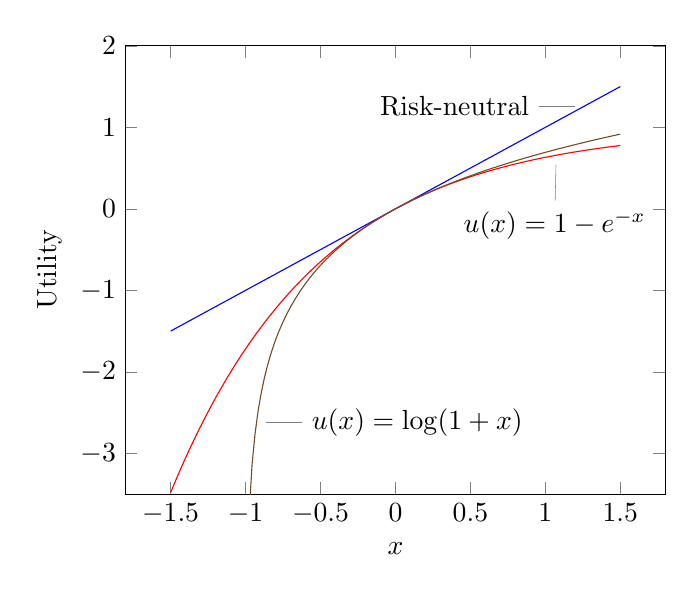
\begin{tikzpicture}
      \begin{axis}[
        xlabel=$x$,
        ylabel=Utility,
        domain=-1.5:1.5,
        samples=150,
        ymin=-3.5
        ]
        \addplot+[mark=none] {x}
        node[pos=0.92, pin={[black]180:Risk-neutral}]{};
        \addplot+[mark=none] {1-exp(-x)}
        node[pos=0.92, pin={[black]-92:$u(x)=1-e^{-x}$}] {};
        \addplot+[mark=none] {ln(1+x)}
        node[pos=0.4, pin={[black]0:$u(x)=\log(1+x)$}] {};
      \end{axis}
    \end{tikzpicture}
    \caption{Comparison of the exponential and logarithmic
      utilities. As $x$ approaches -1 from above, the utility to a logarithmic
      decision maker is modelled to be infinitely bad.
    }\label{fig:example_utilities}
  \end{figure}
\end{example}

For a given utility function that models a decision maker's measure of
benefit for the outcomes of $f$, one can define an ordering
between random variables that decides which of two decisions
$x_1,x_2\in\mathcal{X}$ are better.
\begin{mydef}[Expected utility ordering]
  A utility function $u(x)$ defines an ordering $\preceq$ between random
  variables $X$ and $Y$,
  \begin{equation}
    X\preceq Y \Leftrightarrow \mathbb{E}[u(X)] \leq \mathbb{E}[u(Y)].
  \end{equation}
\end{mydef}
\begin{remark}
  Utility-orderings are preserved by positive affine transformations.
  That is, the ordering defined by $u(x)$ is equivalent to the
  ordering defined by $x\mapsto au(x)+b$ for  $a>0$ and $b\in\mathbb{R}$.
\end{remark}


We can, therefore, formulate a well-defined optimisation problem by
modelling the decision maker's attitude to risk with utility functions.

\begin{problem}[Expected utility]
  The optimal choice to maximise a given utility of $f$ is the
  solution of
  \begin{align}
    x(u)=\argmax_{x\in\mathcal{X}} \mathbb{E}[u(f(x,y))].
  \end{align}
\end{problem}


\subsection{Mean-deviation problems}
The expected utility approach considers the mean outcome of a choice.
After one makes a decision $x\in\mathcal{X}$, the realisation of the
parameter in $\mathcal{Y}$ only occurs once. If there is a large
uncertainty in $f(x,y)$, or, if the distribution is multimodal, the
average value may not be a good representation for the realised value of $f$.
It can, therefore, be useful to take into account some measure of
deviation from the mean of $f$ when $x$ is chosen.
The mean-deviation approach aims to balance the expected value of $f$
with uncertainty represented by a deviation measure.
\begin{mydef}[Deviation measure]
  Let $\mathbb{D}$ be a functional on a linear space of random
  variables which is closed under taking absolute values and contains
  the real numbers.
  Then $\mathbb{D}$ is a deviation measure if
  \begin{enumerate}
  \item $\mathbb{D}[C] = 0$ for any constant $C$, and
  \item $\mathbb{D}[X]>0$ for non-constant random variables $X$.
  \end{enumerate}
\end{mydef}
Deviation measures on $L^2$ random variables were introduced by
\citet{rockafellar2006generalized}, however, the definition used in this thesis
is less strict on the properties of $\mathbb{D}$.

\begin{example}[Deviation measures]
  The classic measure of deviation is the standard deviation.
  Define the $L^p$ norm ${\|X\|}_p := {\left( \mathbb{E}[{|X|}^p]
    \right)}^{1/p}$.
  The standard deviation is
  the particular case $p=2$ of the deviation measures defined by
  the $L^p$-norms,
  \begin{equation}
    X\mapsto
    \|X-\mathbb{E}[X]\|_p.
    \qquad\qquad \text{($L^p$-deviations)}
  \end{equation}

  In some maximisation settings, one might not be worried about
  realisations of $f$ that are larger than its mean, especially if the
  random variable is not symmetric.
  The lower semi-deviation measure only investigates
  worse-than-expected outcomes,
  \begin{align}
    X\mapsto \mathbb{E}[\min(X-\mathbb{E}[X],0)].
    &&\text{(Lower semi-deviation)}
  \end{align}

  One can also combine two deviation-measures in order to capture
  different aspects of a random variable.
  If $\mathbb{D}_1,\dots,\mathbb{D}_k$ are $k$ deviation measures and
  $\lambda_i>0$, then the following
  is also a deviation measure.
  \begin{align}
    \mathbb{D}[X]=\sum_{i=1}^k\lambda_i\mathbb{D}_i[X].
    &&\text{(Weighted deviations)}
  \end{align}
\end{example}


\begin{problem}[Mean-deviation]
  An optimal decision that maximises the expected value of $f$, whilst
  minimising the deviation $\mathbb{D}$ of $f$, is a minimiser to the
  bi-objective optimisation problem
  \begin{align}
    \max_{x\in\mathcal{X}}\{(\mathbb{E}[f(x,y)],\,-\mathbb{D}[f(x,y)])\}.
  \end{align}
\end{problem}
For a given deviation measure that models the decision maker's
need for stability, one can formulate a bi-objective optimisation
problem.
We can approach the bi-objective problem from a multi-objective
optimisation theory point of view and will do so in
\Cref{sec:one_multi-objective}.
The review by \citet{marler2004survey} covers some of the theory,
discusses what optimality means, and introduces approaches to solve
such problems.
A simple approach is to define a single objective function that combines
the expected value with a deviation-penalty, weighted by some
parameter $\lambda>0$. The optimal decision in $\mathcal{X}$ is then
defined as
\begin{equation}\label{eq:mean_dev_weighted}
  x(\mathbb{D},\lambda)=\argmax_{x\in\mathcal{X}}\{\mathbb{E}[f(x,y)]-\lambda
  \mathbb{D}[f(x,y)]\}.
\end{equation}
This implicitly defines an ordering of random variables based on
the functional $X\mapsto \mathbb{E}[X]-\lambda \mathbb{D}[X]$.
If $f$ is nonlinear, then $x(\mathbb{D},\lambda)$ can be unstable to
small changes in $\lambda$. This is illustrated in
\Cref{ex:pareto_disconnected} of \Cref{sec:one_multi-objective}.
Small errors in determining the best
$\lambda$ to represent a decision-maker can cause large changes in
either of the objectives. \citet{marler2004survey} cover
more robust methods.

\subsection{Nonlinear expectations}\label{sec:nonlinear_expectations}
A general framework that covers most of the remaining models
in optimisation under uncertainty makes use of a class of functionals
called nonlinear expectations. The term nonlinear expectation is used
by \citet{peng2010nonlinear} to generalise stochastic calculus to
distributional uncertainty.
The theory was inspired by work in finance for the study of financial
positions using
risk measures, see,
for example, \citet[Ch.~4]{follmer2004stochastic}.
Risk measures are used in a minimisation setting related to losses,
but we will use the term nonlinear expectations in the maximisation
setting. The examples of nonlinear expectations $\mathbb{U}$ considered
in this section give rise to well-known risk measures $\rho$ by using the mapping
$\rho(X) = -\mathbb{U}[X]$.

\begin{mydef}[Nonlinear expectation]
  Let $\mathbb{U}$ be a functional on a linear space of random
  variables which is closed under taking absolute values and contains
  the real numbers.
  Then $\mathbb{U}$ is a nonlinear expectation if
  \begin{enumerate}
  \item $\mathbb{U}[C] = C$ for any constant $C$, and
  \item $\mathbb{U}[X]\leq \mathbb{U}[Y]$ whenever $X\leq Y$ almost surely.
  \end{enumerate}
\end{mydef}
Note that the classic, linear expectation $\mathbb{E}$ also satisfies
the properties of a nonlinear expectation.
A more restricted class of functionals called superlinear expectations
relate to the coherent risk measures from mathematical finance.
\begin{mydef}[Superlinear expectation]
  A nonlinear expectation $\mathbb{U}$ is superlinear if
  \begin{enumerate}
  \item[3.] $\mathbb{U}[X+Y]\geq \mathbb{U}[X] +\mathbb{U}[Y]$ for
    each $X,Y$, and
  \item[4.] $\mathbb{U}[\lambda X] = \lambda\mathbb{U}[X]$ for
    $\lambda\geq 0$.
  \end{enumerate}
\end{mydef}

If $\mathbb{U}$ is a nonlinear expectation
with $\mathbb{U}[X] < \mathbb{E}[X]$ for all non-constant $X$,
then one can
construct a deviation measure with the functional
$\mathbb{D}[X]=\mathbb{E}[X]-\mathbb{U}[X]$.
Further connections between nonlinear expectations and deviation
measures are discussed by \citet{rockafellar2013fundamental}.

\begin{example}[Nonlinear expectations]
  With $\lambda>0$, the functional
  $\mathbb{U}_\lambda[X]=-\frac{1}{\lambda}\log\mathbb{E}[e^{-\lambda
    X}]$, is called an entropic nonlinear expectation.
  It is connected to the exponential utility function $u_\lambda$, since
  $\mathbb{U}_\lambda[X]= u_\lambda^{-1}(\mathbb{E}[u_\lambda(X)])$.

  The worst-case nonlinear expectation on the sample space $\Omega$,
  defined by
  $X\mapsto  \inf_{\omega\in\Omega}X(\omega)$, is superlinear and
  connects optimisation of nonlinear expectations to robust optimisation \citep{ben2009robust}.
  % If there is an attached
  % probability space on $\Omega$,
  % we use the essential infimum.\todo{Define}

  The quantile operator
  $q_\lambda[X] = \inf\{x\mid\mathbb{P}(X\leq x)>
  \lambda\}$, with $\lambda\in[0,1]$, satisfies the properties of a
  nonlinear expectation.
  Note that the operator is not necessarily concave, which has
  implications for the resulting optimisation problem.
  A concave lower bound on the quantile operator is
  the lower super-quantile,
  \begin{equation}\label{eq:def_avar}
    \mathbb{U}_\lambda[X]=\frac{1}{\lambda}\int_0^\lambda q_t[X]\,\dt,
  \end{equation}
  which defines a superlinear expectation for $\lambda\in(0,1]$.
  Another name for the quantile operator is Value at Risk.
  The risk measures related to the lower super-quantile operator are also referred to as
  the Expected Shortfall, Average Value at Risk, and Conditional Value at Risk
  \citep{artzner1999coherent,rockafellar2002conditional,follmer2004stochastic,rockafellar2013fundamental}.
  Their definitions all coincide with~\eqref{eq:def_avar} when the
  cumulative distribution function of $X$ is continuous, however, in
  the general case they handle discontinuities differently.
\end{example}


\begin{problem}[Nonlinear expectation]
  The optimal choice to maximise a nonlinear expectation
  of $f$ is given by
  \begin{align}
    x(\mathbb{U})=\argmax_{x\in\mathcal{X}} \mathbb{U}[f(x,y)].
  \end{align}
\end{problem}

\begin{example}[Lower super-quantile]
  Following \citet{ben2007old}, we can reformulate the lower
  super-quantile optimisation problem arising from~\eqref{eq:def_avar}
  by introducing an auxiliary variable $\eta\in\mathbb{R}$.
  \begin{equation}\label{eq:opt_avar}
    x_{sq}({\gamma})
    =\argmax_{x\in\mathcal{X},\eta\in\mathbb{R}}
    \left\{\eta - \frac{1}{\gamma}\mathbb{E}[\max(\eta-f(x,y),0)]\right\}.
  \end{equation}
  Note that the objective is not necessarily smooth, due to the
  $\max(\eta-f(x,y),0)$ term. Theory of non-smooth optimisation
  can address this but may require sophisticated mathematical techniques, as
  exemplified in \citep{kouri2016risk}.
\end{example}


\section{Different approaches lead to the same decision}\label{sec:one_comparison_orderings}
% The aim of this section is to compare the
% optimisation formulations introduced in the previous section.
Can the mean-deviation formulation give the
same result as the expected utility and nonlinear expectation methods?
In this section we argue that there are cases where they do,
focusing on the mean and standard deviation, exponential
utility, and lower super-quantile.

The exponential utility and lower super-quantile are often more costly
to compute or approximate than the mean and variance, and require a
full description of the distribution of $y$.
Say a given nonlinear expectation $\mathbb{U}$, or utility $u$,
implies that the decision $x^*$ is optimal. Further, assume that we can get a
decision close to $x^*$ from a bi-objective formulation using mean and standard
deviation. The mean-deviation formulation may then be preferable in
practical settings.
This is, for example, illustrated in the articles by
\citet{kouri2016risk} and \citet{alexanderian2017mean}, who address optimisation problems
where each value $y\in\mathcal{Y}$ require the solution to partial
differential equations.
The lower super-quantile approach of \citet{kouri2016risk}
requires the authors to draw samples from $\mathcal{Y}$ and find ways
to smooth the objective,
whilst \citet{alexanderian2017mean} approximate mean and variance
with Taylor series and do not need to sample from $\mathcal{Y}$.


The use of super-quantiles in revenue management has become popular
the last ten years
\citep{wu2014risk,xue2015optimal,zhou2008optimal,ahmed2007coherent}.
All of these articles argue for super-quantiles and dismiss
optimisation formulations that use the mean and standard deviation
on the grounds that they penalise better-than-expected outcomes.
Distributions of profit in revenue management do in practice
have a more significant lower tail than upper tail, due to inventory
restrictions and fixed costs, which alleviates such problems.
None of these references discuss to what extent super-quantiles change the
optimal decisions for their presented problems compared to a
mean-deviation approach. \citet{choi2011multiproduct}
dismiss the mean-deviation problem by formulating it in terms of the weighted sum of mean and
variance, and then argue that the units of these objects do not
coincide.


\subsection{Equivalence for the normal distribution}
If $f(x,y)$ is normally distributed for each value of
$x\in\mathcal{X}$, then the properties of the random variable are fully
described by the mean and variance functions $x\mapsto
\mathbb{E}[f(x,y)]$ and $x\mapsto \mbox{Var}[f(x,y)]$. This
indicates that all the approaches above implicitly define a
choice of ordering for the bi-objective mean-standard deviation
optimisation problem.

\begin{example}[Lower super-quantile]\label{ex:avar_normal}
  Let $X=\mathbb{E}[X]+ \sqrt{\mbox{Var}[X]} Z$ for $Z\sim\mathcal{N}(0,1)$.
  Then the $\gamma$-quantile of $X$ is
  $q_\gamma[X] = \mathbb{E}[X] + \sqrt{\mbox{Var}[X]} q_\gamma[Z]$.
  Thus, the lower super-quantile $\mathbb{U}_\gamma$ of $X$ depends only on
  its mean and variance, with
  \begin{equation}
    \mathbb{U}_\gamma[X] =  \mathbb{E}[X]
    + \sqrt{\mbox{Var}[X]} \mathbb{U}_\gamma[Z].
  \end{equation}
  Note that $\mathbb{U}_\gamma[Z]\leq 0$ for each $\gamma\in(0,1]$,
  with equality only when $\gamma=1$.
  The lower super-quantile optimisation problem is, therefore,
  a special case of the mean-deviation optimisation problem
  with $\mathbb{D}[X]=\sqrt{\mbox{Var}[X]}$,
  using the weighted sum ordering from~\eqref{eq:mean_dev_weighted} and
  $\lambda = -\mathbb{U}_\gamma[Z]$.
\end{example}

\begin{example}[Exponential utility]
  Let $X=\mathbb{E}[X]+ \mathbb{D}[X] Z$, as in \Cref{ex:avar_normal}.
  Then its exponential utility $u$ with parameter $\mu$
  is
  \begin{equation}
    u(X) = 1 - e^{-\mu (\mathbb{E}[X] +
      \mathbb{D}[X] Z)}.
  \end{equation}
  If $f(x,y)$ is normally distributed, the expected utility
  optimisation for $u$ is equivalent to solving
  \begin{equation}
    \min_{x\in\mathcal{X}}  e^{-\mu\mathbb{E}[f(x,y)]}
    \mathbb{E} \left[ e^{-\mu \mathbb{D}[f(x,y)] Z} \right].
  \end{equation}
  In the context of multi-objective optimisation, this arises from
  a particular choice of ordering of the mean-standard deviation
  problem \citep{marler2004survey}.
\end{example}

The review by \citet{nadarajah2014estimation} on estimation methods for
lower super-quantiles provide further evidence that people use
the first two moments of a random variable to estimate nonlinear
expectations for more generic distributions.


\subsection{Finding equivalent mean-deviation formulations}
Consider the decisions that arise from the following
optimisation problems of mean-deviation, exponential utility, and
lower super-quantile $\mathbb{U}_\gamma$.
\begin{subequations}\label{eq:optim_formulations}
  \begin{align}\label{eq:optim_formulations_md}
    x_{md}(\lambda)
    &=\argmax_{x\in\mathcal{X}}\{\mathbb{E}[f(x,y)]-\lambda\sqrt{\mbox{Var}[f(x,y)]}\}
    &\lambda\geq 0,\\\label{eq:optim_formulations_eu}
    % &&\text{(mean-deviation)},\\
    x_{eu}(\mu)
    &=\argmax_{x\in\mathcal{X}}\{
      \mathbb{E}[1-e^{-\mu f(x,y)}]\}
    &\mu>0,\\\label{eq:optim_formulations_sq}
    % &&\text{(exponential utility)},\\
    x_{sq}(\gamma)
    &=\argmax_{x\in\mathcal{X}}
      \{\mathbb{U}_\gamma[f(x,y)]\}
    &\gamma\in(0,1].
    % &&\text{(lower super-quantile)}.
  \end{align}
\end{subequations}
We want to understand whether there are triples $(\lambda,\mu,\gamma)$ that give rise
to the same decisions, $x_{md}=x_{eu}=x_{sq}$, and investigate this in
the following way.
For a given value $\mu>0$ or $\gamma\in(0,1]$, find the minimisers
$\lambda(\mu)$ and $\lambda(\gamma)$ of
\begin{equation}\label{eq:min_xmd_xeu_xsq}
  \min_{\lambda\geq 0}\left\{\frac{{\|x_{md}(\lambda)-x_{eu}(\mu)\|}_2}{{{\|x_{eu}(\mu)}\|}_2}\right\},\quad
  \textnormal{ and}\quad
  \min_{\lambda\geq 0}\left\{\frac{{\|x_{md}(\lambda)-x_{sq}(\gamma)\|}_2}{{{\|x_{sq}(\gamma)}\|}_2}\right\}.
\end{equation}
If the denominators are zero, we minimise the absolute differences instead.
If the minimum is close to zero, it is an indication that either method
can be used to model the risk-preferences of a particular decision maker.
\Cref{fig:util_meandev_2d} shows the result of such an investigation,
and for the particular example considered the differences are small.
In general, it is likely to be examples where the choice of
optimisation formulation matters for the decision. The purpose of this
section is to highlight that one should investigate the structure of
a problem and choose among the computationally tractable options based
on their practical implications instead of solely focusing on
theoretical properties of the different formulations.

\begin{example}[Pricing problem]
  Let us consider situation one of the retail example in
  \Cref{sec:one_motivating_example}, where the product manager wants
  to maximise profit $f(x,y)$, but only knows the distribution of $y$.

  Note that the mean and standard deviation of the profit are
  \begin{equation}
    \mathbb{E}[f(x,y)]
    = \langle x-m_y,q(x) \rangle,\qquad
    \mbox{Var}[f(x,y)]
    = \langle q(x),C_y q(x) \rangle.
  \end{equation}
  Thus, the mean-deviation method with
  $\mathbb{D}[X]=\sqrt{\mbox{Var}[X]}$ has a closed form objective and
  one only needs information about the two first moments of $y$ to solve
  the mean-deviation problem~\eqref{eq:optim_formulations_md}.
  The solution to the expected utility and lower super-quantile
  problems~\eqref{eq:optim_formulations_eu}
  and~\eqref{eq:optim_formulations_sq} require that we approximate the
  objectives, for example, with Monte-Carlo
  \citep{caflisch1998monte}.
  The super-quantile method also needs an extra smoothing step to
  handle the $\max(\eta-f(x,y),0)$ term of~\eqref{eq:opt_avar},
  introducing larger costs and implementational complexity.

  We solve the optimisation problems in~\eqref{eq:min_xmd_xeu_xsq} with
  uniformly spaced values $\mu\in[0,82]$ and $\gamma\in[1/100, 1]$.
  \Cref{fig:util_meandev_2d,fig:cvar_meandev_2d} show the
  corresponding values $\lambda(\mu)$ and $\lambda(\gamma)$, together
  with the difference in the objectives. The values of $\lambda$
  are stable to small changes in $\mu$ and $\gamma$, and the
  reported price differences are unlikely to have an effect when
  the products are priced in-store.
  \begin{figure}[htbp]
    \centering
    \begin{subfigure}[t]{.5\textwidth}
      \includegraphics[width=\textwidth,axisratio=1.3]{util_meandev_3d_x}
    \end{subfigure}%
    \begin{subfigure}[t]{.5\textwidth}
      \includegraphics[width=\textwidth,axisratio=1.3]{util_meandev_3d_l}
    \end{subfigure}
    \caption{The left plot shows the difference between the decision made
      by the mean-deviation and exponential utility methods defined in
      \Cref{eq:optim_formulations}, using the corresponding
      $(\mu,\lambda)$-pairs from the right plot.
      The discontinuity in the left plot corresponds to an abrupt
      change in $x(\mu)$.%, and the corresponding $\lambda$ actually
      % drops slightly, although this is not visible.
    }\label{fig:util_meandev_2d}
  \end{figure}

  \begin{figure}[hbtp]
    \centering
    \begin{subfigure}[t]{.5\textwidth}
      \includegraphics[width=\textwidth,axisratio=1.3]{cvar_meandev_3d_x}
    \end{subfigure}%
    \begin{subfigure}[t]{.5\textwidth}
      \includegraphics[width=\textwidth,axisratio=1.3]{cvar_meandev_3d_l}
    \end{subfigure}
    \caption{The left plot shows the difference between the decision made
      from the mean-deviation and super-quantile methods defined in
      \Cref{eq:optim_formulations}, using the corresponding
      $(\gamma,\lambda)$-pairs from the right plot.
    }\label{fig:cvar_meandev_2d}
  \end{figure}
\end{example}




\section{Randomness and
  constraints}\label{sec:one_randomness_constraints}
We briefly discuss the situation arising from the
second decision problem posed in \Cref{sec:one_motivating_example},
where the decision maker wants to maximise revenue but ensure that
profit is positive.

Introduce a deterministic objective $g:\mathcal{X}
\to\mathbb{R}$. In the deterministic setting, with a known parameter
$y\in\mathcal{Y}$, one often considers problems of the form
\begin{align}
  \min_{x\in\mathcal{X}}\{g(x)\mid f(x,y)\geq f_{\textnormal{min}} \},\;
  \text{ for some } f_{\textnormal{min}}\in\mathbb{R}.
\end{align}
Then $f\geq f_{\textnormal{min}}$ is considered a constraint, which restricts the
decision space to $\{x\in\mathcal{X}\mid f(x,y)\geq f_{\textnormal{min}}\}$.
When there is uncertainty about the right parameter-value, this set is
not defined at the time of the decision but depends on future knowledge
of the parameter.

In the engineering community, it is popular to
reinterpret non-deterministic ``constraints'' as deterministic via
expected utilities, mean-deviation methods or nonlinear
expectations
\citep{rockafellar2007coherent,rockafellar2015engineering}.
Such a reinterpretation defines an acceptance set $\mathcal{A}$
which represents what a decision maker deems to be feasible in a
risk-adjusted way and results in the optimisation problem
$\min_{x\in\mathcal{A}} g(x)$.
The acceptance set approach was one of the motivations for a formal
framework for risk measures introduced by \citet{artzner1999coherent}.
\begin{example}[Acceptance sets]
  Popular choices of acceptance sets for the constraint $f(x,y)\geq
  f_{\textnormal{min}}$ are
  \begin{align}
    \mathcal{A}&=\{x\in\mathcal{X} \mid
                 \mathbb{E}[f(x,y)]\geq f_{\textnormal{min}}\},
    &\textnormal{(Expectation)}\\
    \mathcal{A}&=\{x\in\mathcal{X} \mid
                 \inf_{\omega\in\Omega}f(x,y(\omega))\geq
                 f_{\textnormal{min}}\},
    &\textnormal{(Worst-case)}\\
    \mathcal{A} &= \{x\in\mathcal{X}\mid
                  \mathbb{P}(f(x,y)\geq f_{\textnormal{min}})\geq \epsilon\},
                  \text{ given }\epsilon\in(0,1).
    &\textnormal{(Quantile)}
  \end{align}
\end{example}

The acceptance set approach treats what was previously considered a
hard constraint in terms of marginalised values that allow decisions $x\in\mathcal{X}$
that may violate the originally intended constraint for some values of the random
variable $y$. We believe that a better approach is to address this
properly by modelling the trade-off between $g(x)$ and the outcomes of $f(x,y)$,
which is a multi-objective optimisation approach.

\section{Multi-objective optimisation}\label{sec:one_multi-objective}
% \todo[inline]{Show that mean-std of revenue with uncertain sales
% generates a non-convex Pareto front (\textbf{BAD for weighted sum
% approach}). Mean-Var should work
% }
Competing objectives often appear in a decision process, and the chapter
has already made multiple references to multi-objective optimisation.  Assume
there are $m$ competing objectives
$f_1,\dots,f_m:\mathcal{X}\to\mathbb{R}$ that we wish to
minimise\footnote{We choose to work within a minimisation-framework
  for the multi-objective theory in order to follow the standards in
  optimisation literature. Any objective $f_i$ that is to be maximised
  can be redefined by $f_i\leftarrow -f_i$.} over the decision space
$\mathcal{X}$. The two main challenges that arise are how to understand
the trade-offs between the objectives, and to define an ordering
between decisions $x\in\mathcal{X}$.  One approach to the first
challenge is to find the Pareto front, or efficient
frontier, of the objectives, which we cover in
\Cref{sec:multi_pareto_front}. The second challenge is more difficult,
as it involves modelling the decision maker's preferences.

Relevant concepts for multi-objective optimisation are defined in
\Cref{sec:multi_terminology}.  The main contribution from this section
is a software package that lets users formulate
multi-objective optimisation problems.  An example in
\Cref{sec:one_multijump} shows how it is used to create the data for
the figures in this section.  The package approximates the Pareto
front with
three methods: Weighted sums, objective
constraints, and the Normal Boundary Intersection method covered in
\Cref{sec:multi_pareto_front}.  A broader range of
approaches to multi-objective optimisation can be found in the survey
by \citet{marler2004survey}.  The multi-objective ordering problem is
discussed in \Cref{sec:multi_apriori}, where it is argued that an
approximation of a decision maker's preferences for multiple
objectives can be made by combining the objectives' utilities.
% In an
% optimisation setting involving randomness, one might already have
% defined utility functions for different objectives, so multiple
% objectives easily fit within the existing theory.


\subsection{Terminology}\label{sec:multi_terminology}
A key concept for multi-objective optimisation is the partial
ordering of outcomes known as Pareto dominance. If a decision leads to
an outcome that is not dominated by any other feasible outcome, it is
optimal in the Pareto sense.
\begin{mydef}[Pareto optimality]
  A point $x\in\mathcal{X}$ is Pareto optimal for the problem
  \begin{equation}
    \min_{x\in\mathcal{X}}\{f_1(x),\dots,f_m(x)\}
  \end{equation}
  if there is no
  $x^*\in\mathcal{X}$ such that
  \begin{align}
    f_i(x^*)&\leq f_i(x) &&\text{ for all } i = 1,\dots,m, \text{ and}\\
    f_j(x^*)&<f_j(x) &&\text{ for at least one } j \in \{1,\dots,m\}.
  \end{align}
\end{mydef}
Pareto optimality, therefore, means that we cannot decrease the value of
one objective without increasing another.
The point $x$ is locally Pareto optimal if it is Pareto optimal in
some neighbourhood around $x$. \Cref{fig:pareto_local_disconnected}
shows an example of both Pareto and locally Pareto optimal points.
\begin{mydef}[Pareto front]
  Define $F(x) = (f_1(x),\dots,f_m(x))$.
  The Pareto front, or efficient frontier $\mathcal{P}\subset
  \mathbb{R}^m$, is the set of
  Pareto optimal objective values,
  \begin{align}
    \mathcal{P} = \{F(x) \mid x \text{ is Pareto optimal}\}.
  \end{align}
\end{mydef}

\begin{example}[Two-dimensional Pareto front]
  \Cref{fig:multi_map} and \Cref{fig:pareto_local_disconnected}
  provide visual representations of the
  multi-objective concepts for two-dimensional problems
  $F:\mathcal{X}\to\mathbb{R}^2$.
  \begin{figure}[htbp]
    \centering
    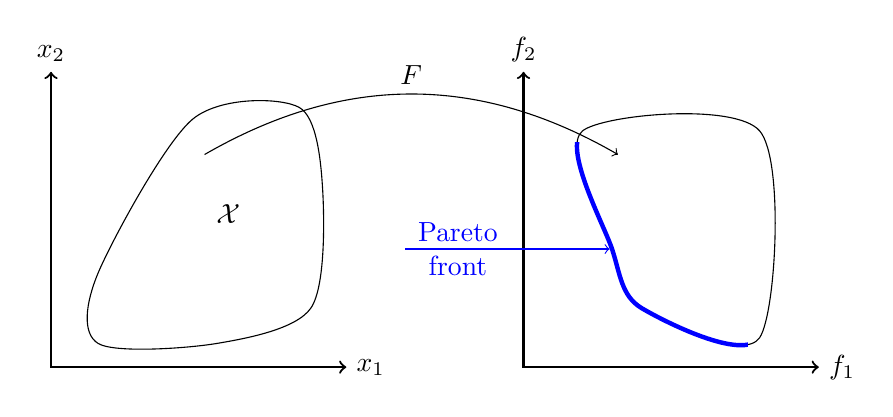
\begin{tikzpicture}[scale=1.5]
      \coordinate (d0) at (0,0);
      \coordinate (d1) at (2.5,0);
      \coordinate (d2) at (0,2.5);
      \coordinate (f0) at (4,0);
      \coordinate (f1) at (6.5,0);
      \coordinate (f2) at (4,2.5);
      % \draw[help lines,step=.5] (0,0) grid (6,3.5);
      \draw [<->,thick] (d2) node (yaxis) [above] {$x_2$}
      |- (d1) node (xaxis) [right] {$x_1$};
      \draw plot [smooth cycle] coordinates
      {(0.4,.2)(1.4,.2)(2.2,.5)(2.3,1.5)(2.1,2.2)(1.2,2.1)(0.4,0.8)} node
      at (1.5,1.3) {$\mathcal{X}$};

      \path[->] (1.3,1.8) edge [bend left] node[above] {$F$} (4.80,1.8);
      \draw [<->,thick] (f2) node (yaxis) [above] {$f_2$}
      |- (f1) node (xaxis) [right] {$f_1$};
      \draw plot [smooth cycle] coordinates
      {(6,0.25) (6,2) (4.5,2) (4.75, 1) (5,0.5)};
      \begin{scope}
        \clip (4,0) rectangle (5.9,1.9);
        \draw[ultra thick, blue] plot [smooth cycle] coordinates
        {(6,0.25) (6,2) (4.5,2) (4.75, 1) (5,0.5)};
      \end{scope}
      \path[->, color=blue] (3.,1) edge node[left,color=blue,align=center] {Pareto\\front} (4.73,1);
    \end{tikzpicture}
    \caption{Pareto concepts for a mapping $F(x)=(f_1(x),f_2(x))$.
      The Pareto front is visualised by the bold line segment on the
      image $F(\mathcal{X})$.
    }\label{fig:multi_map}
  \end{figure}

  \begin{figure}[htb]
    \centering
    \begin{tikzpicture}
      \begin{axis}[width=0.6\textwidth, axis equal image,
        xlabel=$f_1$,
        ylabel=$f_2$,
        domain=0.4:4.6,
        ]
        \addplot [samples=50,name path=A,domain=0.4:4.6,blue,draw opacity=0.1]
        {5*exp(-x)+2*exp(-0.5*(x-3)^2)};
        \path [name path=B]
        (0.4,3.45) -- (4.6,3.45);
        % (\pgfkeysvalueof{/pgfplots/xmin},\pgfkeysvalueof{/pgfplots/ymax}) --
        % (\pgfkeysvalueof{/pgfplots/xmax},\pgfkeysvalueof{/pgfplots/ymax});
        \addplot [blue, fill opacity = 0.1] fill between [of=A and B, soft clip={domain=0.4:4.6}] ;
        \addplot[mark=none, domain=0.4:1.55, ultra thick]
        {5*exp(-x)+2*exp(-0.5*(x-3)^2)}
        node[pos=0.8, pin={[black]-100:Pareto}]{};
        \addplot[mark=none, domain=3.65:4.6, ultra thick]
        {5*exp(-x)+2*exp(-0.5*(x-3)^2)}
        node[pos=0.6, pin={[black]-160:Pareto}]{};
        \addplot[mark=none,domain=2.825:3.65,dashed, thick]
        {5*exp(-x)+2*exp(-0.5*(x-3)^2)}
        node[pos=0.4, pin={[black, pin edge={solid}]90:Locally
          Pareto}]{};
        \node [] at (axis cs:1.5,3) {$F(\mathcal{X})$};
      \end{axis}
    \end{tikzpicture}
    \caption{A disconnected Pareto front of a continuous function $F$
      that also admits locally Pareto optimal points.
    }\label{fig:pareto_local_disconnected}
  \end{figure}
\end{example}




\begin{example}[Retail application]\label{ex:retail_pareto}
  Consider the model from the retail problem described in
  \Cref{sec:one_motivating_example}.
  The Pareto front can be used in the retail setting in order to understand the
  trade-offs between different objectives.
  We consider two situations, both illustrated in
  \Cref{fig:pareto_std_prof_rev}.
  First, say the manager wants to understand the balance between
  maximising expected profit and minimising the profit standard
  deviation.
  Second, the Pareto front can tell how much an increase in revenue
  decreases the expected profit.
  \begin{figure}[htbp]
    \centering
    \begin{subfigure}[h]{.5\textwidth}
      \begin{tikzpicture}
        \begin{axis}[width=0.9\textwidth,
          xlabel=Standard deviation,
          ylabel=Expected profit,
          xtick={0, 0.005, 0.01},
          scaled ticks = false,
          xticklabel style={
            /pgf/number format/precision=3,
            /pgf/number format/fixed,
            % /pgf/number format/fixed zerofill,
          }
          ]
          \addplot[thick] table {./data/pareto_std_prof_3_nbi.dat};
        \end{axis}
      \end{tikzpicture}
    \end{subfigure}%
    \begin{subfigure}[h]{.5\textwidth}
      \begin{tikzpicture}
        \begin{axis}[width=0.9\textwidth,
          xlabel=Revenue,
          ylabel=Expected profit]
          \addplot[thick] table {./data/pareto_prof_rev_nbi.dat};
        \end{axis}
      \end{tikzpicture}
    \end{subfigure}
    \caption{The two plots show the Pareto front between two competing
      objectives. The left figure compares the expected profit of three
      products, compared to the standard deviation of profit.
      On the right, one can see the trade-offs that are made between
      a risk-neutral profit maximisation and a revenue maximisation.
      The code used to generate the left Pareto front is given in
      \Cref{lst:multijump} later in the chapter.
    }\label{fig:pareto_std_prof_rev}
  \end{figure}
  % We make two observations from the Pareto fronts in
  % \Cref{fig:pareto_std_prof_rev}.
  % Reducing the standard deviation has an order of magnitude higher
  % cost on expected value in the middle of the Pareto front, and a
  % better trade-off is likely to be closer to the top-right region.
  % There is a sharp drop in expected profit near
  % the minimal standard deviation, so the gain from decreasing the risk is
  % potentially larger than the losses of expected profit in this region.
  % Relative changes in revenue have a much larger impact on maximum expected
  % profit compared to changing the standard deviation.
\end{example}

\begin{mydef}[Convexity]
  The Pareto-front is said to be convex if the following set is convex.
  \begin{align}
    \overline{\mathcal{P}} = \{t\in\mathbb{R}^m\mid F(x)\leq t \text{ for
    some feasible } x\}.
  \end{align}
\end{mydef}

\begin{example}[Convexity]
  The pricing problems in \Cref{ex:retail_pareto} represent convex Pareto
  fronts.
  An example of a non-convex Pareto front is shown in
  \Cref{fig:pareto_local_disconnected}.
\end{example}

Algorithms for approximating the Pareto front
often make use of particular points describing extremal
values of the objectives.
\begin{mydef}
  Denote $\underline{x_i}$ as the individual minimiser of $f_i$, and
  $\underline{f_i}=f_i(\underline {x_i})$.
  The point $\underline{F}=(\underline{f_1},\dots,\underline{f_m})$
  is the vector containing all individual minima.
  Define the worst outcome for $f_i$ on the Pareto front as
  $\overline{f_i}=\max_{1\leq j\leq m}\{f_i(\underline{x_j})\}$.
  The point  $\overline{F} =
  (\overline{f_1}, \dots, \overline{f_m})$ is the vector containing
  all the worst outcomes.
  % The bounding box is the hypercube bounded below and above by the
  % utopia and nadir points.
\end{mydef}

\begin{example}[Two-dimensional extremal points]
  \Cref{fig:pareto_drawing} illustrates an example of the points
  $\underline{F}$ and $\overline{F}$ %, together with the bounding box
  for a two-dimensional problem $F:\mathcal{X}\to\mathbb{R}^2$.
  \begin{figure}[htbp]
    \centering
    \includegraphics[width=0.5\textwidth]{pareto_drawing}
    \caption{An example Pareto front $\mathcal{P}$ of two
      objectives. The points $\underline{F}$ and $\overline{F}$
      represent the
      lower and upper bound of what values
      $f_1$ and $f_2$ can take on $\mathcal{P}$.}\label{fig:pareto_drawing}
  \end{figure}
\end{example}

\subsection{Approximating the Pareto front}\label{sec:multi_pareto_front}
The Pareto front contains all the information about trade-offs between the
objectives. A decision $x$ to the multi-objective problem
should be a Pareto optimal point, so the
optimisation problem becomes one of searching over the set
$\mathcal{P}$ of co-dimension one. If $\mathcal{X}$ or the objectives are non-convex,
$\mathcal{P}$ can have non-convex regions and be
disconnected.
There are several ways to approximate the Pareto front. The simplest
methods use a weighted sum or vary constraints on the objectives.

\begin{mydef}[Weighted sums]
  For $\lambda \in {[0,1]}^m$ with $\sum_{j=1}^m\lambda_j = 1$, solve
  \begin{equation}
    \min_{x\in\mathcal{X}} \sum_{j=1}^m \lambda_i f_i(x).
  \end{equation}
\end{mydef}
The weighted sum method explores the Pareto front by solving a series
of sub-minimisation problems for the function $\sum_{i=1}^m\lambda_i f_i$.
The $\lambda_i$ represent the relative weighting of each
objective. By varying $\lambda$  we may find new points on the Pareto front.
This approach often works better if the objectives are normalised by the
mapping $f_i\leftarrow (f_i-\underline
{f_i})/(\overline{f_i}-\underline{f_i})$.
There are two major problems with the weighted sum approach. First,
it cannot find Pareto points on non-convex parts of the Pareto
front \citep{messac2000aggregate}.
Second, when the objectives are nonlinear, the solution to the
optimisation problem reacts nonlinearly to changes in $\lambda$.
The Pareto front approximation can, therefore, miss out important
information, and will
have a non-uniform spread of points, as illustrated in
\Cref{fig:pareto_disconnected_ws}.

\begin{mydef}[Constraint method]
  Choose
  $\epsilon_i\in(\underline{f_i},\overline{f_i})$ for $i=2,\dots,m$, and
  solve the minimisation problem
  \begin{equation}\label{eq:pareto_constraint_method}
    \min_x\{f_1(x)\mid f_i(x)\leq \epsilon_i,\, i=2,\dots,m\}.
  \end{equation}
\end{mydef}
The constraint method can find Pareto points in non-convex regions of
$\mathcal{P}$, and gives us control of the spread of points on the Pareto front
along the axes of $f_2,\dots,f_m$. In general, the points will not be
uniformly distributed along the $f_1$-axis.

The Normal Boundary Intersection (NBI) method by \citet{das1998normal} can
create a more uniform spread of the Pareto points in both convex and
non-convex regions of the Pareto front. Its optimisation problem
formulation makes use of the convex hull of the individual minima
(CHIM), defined below.
\begin{mydef}[Convex hull of individual minima (CHIM)]
  Define a matrix $\Phi\in\mathbb{R}^{m\times m}$ with columns
  $\Phi_j = F(\underline{x_j})-\underline{F}$.
  The CHIM is the set
  \begin{equation}\textstyle
    \{\Phi\beta + \underline{F} \mid \beta\in{[0,1]}^m,\;\sum_{j=1}^m\beta_j = 1\}.
  \end{equation}
\end{mydef}

\begin{example}
  \Cref{fig:nbi_drawing2} provides an example of the CHIM for a
  bi-objective problem $F:\mathcal{X}\to\mathbb{R}^2$.
  \begin{figure}[htbp]
    \centering
    \includegraphics[width=0.5\textwidth]{nbi_drawing2}
    \caption{The Normal Boundary Intersection method. It traces out the
      Pareto front by moving from points of the CHIM along the normal
      direction $\hat n$.}\label{fig:nbi_drawing2}
  \end{figure}
\end{example}

\begin{mydef}[Normal Boundary Intersection]
  Let $\hat{n}$ denote the unit normal to the CHIM pointing in the
  direction of smaller values in $\mathbb{R}^m$.
  Given $\beta\in{[0,1]}^m$ such that
  $\sum_{j=1}^m\beta_j=1$, solve
  \begin{equation}
    \max_{x\in\mathcal{X},\,t\in\mathbb{R}} \{t \mid \Phi\beta +
    t\hat{n} = F(x) - \underline{F}\}.
  \end{equation}
\end{mydef}

\begin{example}[Comparison of Pareto front
  approximations]\label{ex:pareto_disconnected}
  We will now investigate the approximations of the Pareto
  front on a toy example using the three different methods.
  Define the function
  $F:{[0,5]}^2\to\mathbb{R}^2$ by $F=(f_1,f_2)$, with $f_i(x)=x_i$.
  Consider the bi-objective problem
  \begin{align}
    \min_{x\in{[0,5]}^2}\{F(x)\mid
    5e^{-x_1}+2e^{-\frac{1}{2}{(x_1-3)}^2} \leq x_2\}.
  \end{align}
  The Pareto front is disconnected and contains points that are
  locally, but not globally, Pareto optimal. The Pareto front and the
  image of $F(x)$ are shown in \Cref{fig:pareto_local_disconnected} for
  the restricted domain $\mathcal{X}_{\textnormal{r}}=\{x\in {[0.4,4.6]}^2 \mid
  5e^{-x_1}+2e^{-\frac{1}{2}{(x_1-3)}^2} \leq x_2\}$.

  All the three methods, weighted sum, varying constraints, and NBI, define
  subproblems parameterised by a value $\lambda\in{[0,1]}^{m}$. Without any
  a priori knowledge or adaptivity, we wish to approximate the Pareto front
  with \num{40} uniformly spaced parameter values.
  In \Cref{fig:pareto_disconnected} one can see how the three methods
  perform in creating a uniform spread of points along the
  Pareto front.
  \begin{figure}[htbp]
    \centering
    \begin{subfigure}[t]{.5\textwidth}
      \begin{tikzpicture}
        \begin{axis}[width=0.9\textwidth,
          xlabel=$f_1$,
          ylabel=$f_2$,
          ]
          \addplot[only marks, mark size=0.6] table
          {./data/pareto_disconnected_nbi_eq.dat};
          \addplot[mark=none, domain=0:1.55, orange]
          {5*exp(-x)+2*exp(-0.5*(x-3)^2)};
          \addplot[mark=none, domain=3.65:5, orange]
          {5*exp(-x)+2*exp(-0.5*(x-3)^2)};
        \end{axis}
      \end{tikzpicture}
      \caption{NBI}\label{fig:pareto_disconnected_nbi_eq}
    \end{subfigure}%
    \begin{subfigure}[t]{.5\textwidth}
      \begin{tikzpicture}
        \begin{axis}[width=0.9\textwidth,
          xlabel=$f_1$,
          ylabel=$f_2$,
          ]
          \addplot[mark=none, domain=0:1.55, orange]
          {5*exp(-x)+2*exp(-0.5*(x-3)^2)};
          \addplot[mark=none, domain=3.65:5, orange]
          {5*exp(-x)+2*exp(-0.5*(x-3)^2)};
          \addplot[only marks, mark size=0.6] table
          {./data/pareto_disconnected_eps.dat};
        \end{axis}
      \end{tikzpicture}
      \caption{Varying constraint on $f_2$}
    \end{subfigure}\\[1em]
    \begin{subfigure}[t]{.5\textwidth}
      \begin{tikzpicture}
        \begin{axis}[width=0.9\textwidth,
          xlabel=$f_1$,
          ylabel=$f_2$,
          ]
          \addplot[mark=none, domain=0:1.55, orange]
          {5*exp(-x)+2*exp(-0.5*(x-3)^2)};
          \addplot[mark=none, domain=3.65:5, orange]
          {5*exp(-x)+2*exp(-0.5*(x-3)^2)};
          \addplot[only marks, mark size=0.6] table
          {./data/pareto_disconnected_ws.dat};
          \draw [red] (axis cs:0,5) circle [radius=0.09]
          node[right] {7 points};
          \draw [red] (axis cs:5,0.3) circle [radius=0.09]
          node[left] {16 points\;\;};
        \end{axis}
      \end{tikzpicture}
      \caption{Weighted sums}\label{fig:pareto_disconnected_ws}
    \end{subfigure}
    \caption{Approximations of a disconnected Pareto front, together
      with the Pareto front in orange.
      The NBI algorithm finds points that are not Pareto optimal, but
      is otherwise providing the best approximation of the Pareto front.
    }\label{fig:pareto_disconnected}
  \end{figure}

  The weighted sum method provides the least information about the
  Pareto front, and many of the points are clustered on top of each
  other at the two ends of the Pareto front.
  The varying constraint method misses a portion of the Pareto front,
  and instead produces some points that are only
  locally Pareto optimal. This is because the underlying optimisation
  algorithm for each sub-problem finds local solutions
  to~\eqref{eq:pareto_constraint_method}.
  NBI provides a uniform spread that gives us the most
  information for the same number of sub-problem optimisations,
  however, it also produces some points that are not locally
  Pareto optimal.
\end{example}

When the Pareto front is disconnected, \Cref{ex:pareto_disconnected}
shows that the NBI method can find
points that are not locally Pareto optimal.
We can modify the method so that the method produces
locally optimal points.
\begin{mydef}[NBI extension]
  Given $\beta\in{[0,1]}^m$ with $\sum_{j=1}^m\beta_j=1$,
  solve
  \begin{equation}
    \max_{x\in\mathcal{X},\,t\in\mathbb{R}} \{t \mid \Phi\beta +
    t\hat{n} \geq F(x) - \underline{F}\}.
  \end{equation}
\end{mydef}

\begin{example}[Disconnected Pareto front with NBI extension]\label{ex:pareto_disconnected_nbi_ineq}
  Consider the bi-objective optimisation problem from
  \Cref{ex:pareto_disconnected}.
  \Cref{fig:pareto_disconnected_nbi_ineq}
  shows $\num{40}$ points approximating the Pareto front using the NBI
  extension, which are all locally Pareto optimal.
  \begin{figure}[htb]
    \centering
    \begin{tikzpicture}
      \begin{axis}[width=0.45\textwidth,
        xlabel=$f_1$,
        ylabel=$f_2$,
        ]
        \addplot[mark=none, domain=0:1.55, orange]
        {5*exp(-x)+2*exp(-0.5*(x-3)^2)};
        \addplot[mark=none, domain=3.65:5, orange]
        {5*exp(-x)+2*exp(-0.5*(x-3)^2)};
        \addplot[only marks, mark size=0.6] table
        {./data/pareto_disconnected_nbi_ineq.dat};
        \draw [red] (axis cs:1.59,1.75) circle [radius=0.09]
        node[below] {4 points};
      \end{axis}
    \end{tikzpicture}
    \caption{The NBI extension creates only locally Pareto optimal
      points, in contrast to the NBI method, as seen in
      \Cref{fig:pareto_disconnected_nbi_eq}.
      There are four points lying on top of each other
      because the current algorithm is not adaptive.}\label{fig:pareto_disconnected_nbi_ineq}
  \end{figure}
\end{example}

The NBI method is a special case of the scalarization methods for
vector-optimisation formulated by
\citet{pascoletti1984scalarizing}. The NBI extension fits within the
Pascoletti-Serafini framework in such a way that it guarantees local
Pareto optimality. \Cref{fig:pareto_disconnected,fig:pareto_disconnected_nbi_ineq} show
issues that arise with a disconnected Pareto front.
The NBI extension implemented in the package MultiJuMP, described in
\Cref{sec:one_multijump}, finds the same point multiple times on the
border of disconnected components of the Pareto front, as illustrated
in \Cref{fig:pareto_disconnected_nbi_ineq}.
\citet{eichfelder2009adaptive} has devised an adaptive algorithm based
on Pascoletti-Serafini scalarization that can better handle non-convex
and disconnected Pareto fronts.



\subsection{Ordering decision points a priori}\label{sec:multi_apriori}
Up to now we have described a process for making a decision
$x\in\mathcal{X}$ that involves approximating the Pareto
front.
The cost of the approximation stage increases exponentially with the
number of objectives. The preferred position on the Pareto front is
subjective and prone to change depending on the presentation of
$\mathcal{P}$. With more than two objectives, it is difficult to
present the Pareto front without losing some information.
Given the same Pareto front, presented in
$k$ different ways, the variation of decisions $x^1,\dots,x^k$ is likely to
increase with the number of objectives.
Ideally one would like to create an ordering between decisions so
that the optimal decision is the same every time the same optimisation
problem is run.

Simple approaches to creating an ordering include the weighted sum
and constrained objectives methods.
With weighted sums, the ordering will be based on
an ordering defined by the function $u(x)=\sum_{i=1}^n\lambda_if_i(x)$.
The challenge is then to decide the relative weights of the objectives. The
nonlinear response of $\lambda$ in the weighted sum method means that
the defined ordering can be unstable to small perturbations of $\lambda$.
One can instead define upper bounds for $f_2,\dots,f_m$ and minimise
$f_1$.
Given the upper bounds
$\epsilon_i\in[\underline{f_i},\overline{f_i}]$,
the ordering is only on the value of the first objective.
Small changes in $\epsilon$ can turn an optimal decision $x$
infeasible. There is no room for the optimisation algorithm to
look at trade-offs between objectives, although one could get some
understanding of trade-offs from the
Lagrange multipliers of the constraints.

To define an ordering of decisions, one should find a way to express
the total value $u:\mathbb{R}^m\to\mathbb{R}$ of the multi-objective
function $F$. The survey by \citet{marler2004survey} describes
different choices of the function $u$ that has been used in the literature.
\citet{messac1996physical} attempts to create a total value function
with an approach he calls Physical Programming. The decision
maker defines what a ``desirable'', ``tolerable'',
``undesirable'' value corresponds to for each objective. The implementation of this method
is much more complicated than the other approaches considered but
may give us an easier framework to approximate a decision maker's preferences.

The total value function $u(F)$ can be thought of as a
multivariate utility function. To ensure that an optimal decision
according to $u$ is also Pareto optimal, impose that $u$ is
strictly increasing in all of its arguments.
If the decision problem involves randomness, one may already have
tried to model the decision maker's risk-aversion for each objective.
With the expected utility approach to risk-aversion, that would mean
that utility functions $u_i$ are readily available. One can then make
a simple approximation of
the total value $u(F)$ with the mapping $F\mapsto \sum_{i=1}^n u_i(f_i)$.
If the $u_i$ are concave, then $u$ defines a multivariate risk-averse
utility \citep[Sec. 2.3.2]{campi2011multivariate}.
This could provide a good first approximation to orderings in
multi-objective optimisation problems involving randomness.


\subsection{Approximating Pareto fronts with
  MultiJuMP}\label{sec:one_multijump}
As part of the work on multi-objective optimisation, I have created a
software package called MultiJuMP.  It is available online at
\url{https://github.com/anriseth/MultiJuMP.jl.git}.  MultiJuMP
approximates Pareto fronts in a numerical solver-independent
environment, using the four methods discussed in
\Cref{sec:multi_pareto_front}.  The package is written in the Julia
programming language \citep{bezanson2017julia}, and based on the
mathematical programming modelling package JuMP
\citep{dunning2017jump}. It separates the challenge of expressing an
optimisation problem from the algorithm-specific decision of solving
the problem. \Cref{lst:multijump} shows an example of how to set up a
multi-objective optimisation model with the MultiJuMP routines. The
code works for any number of objectives, however, visualising a Pareto
front for more than three objectives becomes difficult.
\begin{listing}[htbp]
  \inputminted{julia}{./include/multijump.jl}
  \caption{Code used to generate one of the figures in
    \Cref{ex:retail_pareto}.
    The functions \mintinline{julia}{MultiModel()},
    \mintinline{julia}{getMultiData()},
    \mintinline{julia}{SingleObjective()} and \mintinline{julia}{solve()}
    were created as part of the work on MultiJuMP.
  }\label{lst:multijump}
\end{listing}


\biblio{} % Bibliography when standalone
\end{document}

%%% Local Variables:
%%% mode: latex
%%% TeX-master: t
%%% TeX-command-extra-options: "--shell-escape"
%%% TeX-command-extra-options: "-shell-escape"
%%% End:
